
\chapter{Hit Discovery via Unsupervised Learning of Fragment-Protein Complexes} \label{ch:fresco}

% ... This chapter ...

% The process of finding molecules that bind to a target protein is a challenging first step in drug discovery. Crystallographic fragment screening is a strategy based on elucidating binding modes of small polar compounds and then building potency by expanding or merging them. Recent advances in high-throughput crystallography enable the screening of large fragment libraries, reading out dense ensembles of fragments spanning the binding site. However, fragments typically have low affinity thus the road to potency is often long and fraught with false starts. Here, we take advantage of high-throughput crystallography to reframe fragment-based hit discovery as a denoising problem -- identifying significant pharmacophore distributions from a fragment ensemble amid noise due to weak binders -- and employ an unsupervised machine learning method to tackle this problem. Our method screens potential molecules by evaluating whether they recapitulate those fragment-derived pharmacophore distributions. We retrospectively validated our approach on an open science campaign against SARS-CoV-2 main protease (Mpro), showing that our method can distinguish active compounds from inactive ones using only structural data of fragment-protein complexes, without any activity data. Further, we prospectively found novel hits for Mpro and the Mac1 domain of SARS-CoV-2 non-structural protein 3. More broadly, our results demonstrate how unsupervised machine learning helps interpret high throughput crystallography data to rapidly discover potent chemical modulators of protein function. 

% \section{Introduction}

Hit detection is a key step in the early stages of the drug discovery process following the identification of a biological target of interest \cite{Hughes2011Principles}. A `hit' compound acts as the starting point for the drug design process where the chemical structure of the hit is progressively optimised towards a candidate drug. Approaches towards hit detection generally involve screening large libraries of compounds, both experimentally and computationally.

% Approaches towards hit detection generally involve the screening of libraries of compounds. For example, in high throughput screening (HTS) often hundreds of thousands of chemical compounds are synthesised and tested, requiring substantial resources as well as complex logistics. While experimental techniques such as DNA-Encoded libraries are being developed to increase the efficiency of large-scale compound screening \cite{GirondaMartinez2021DNALibrary}, there has been a growing push towards conducting hit detection computationally instead to decrease the cost and accelerate this step of the drug discovery process \cite{?}. 

% In this approach, known as virtual screening, a computational scoring function is used to estimate the potency of a compound. After computing the scores for all of the compounds in a library, only those ranked highly by the scoring function are chosen for synthesis and experimental validation. Currently, the predominant scoring function used to conduct a virtual screen is molecular docking. In molecular docking, the 3D conformation of a ligand and the target are explicitly modelled and a physics-based simulation of the binding process is conducted, with the calculated energy of the bound ligand as the score. Although this approach has yielded success \cite{Lyu2019UltraLargeDocking, Alon2021SigmaTwo}, correctly performing molecular docking is non-trivial and the deficiencies of molecular docking for bioactivity prediction are well-documented \cite{Llanos2021StrengthsAndWeaknesses, Macip2022HasteMakesWaste}.

% An alternative to these methodologies is fragment-based drug discovery (FBDD). In this approach, a library of very low molecular weight compounds (`fragments' typically less than 18 nonhydrogen atoms \cite{David2017FBLD}) is screened at high concentrations alongside the generation of bound fragment-protein structures via X-ray crystallography or cryo-EM. By obtaining these experimental structures and examining the binding interactions between individual fragments with protein residues, fragments can be used as building blocks for larger molecules by linking or merging disparate fragments in order to increase potency. Conceptually, FBDD is based on a coarse-graining of fragments to specific moieties or groups that are associated with interactions with the target, to maintain and optimise these interactions in larger molecules.

One of these methodologies is fragment-based drug design (FBDD). In this approach, protein crystals are soaked with high concencration of very low molecular weight compounds (`fragments' with typically less than 18 non-hydrogen atoms \cite{David2017FBLD}) and the resulting protein-fragment complexes are resolved with X-ray crystallography. A fragment screening approach is more likely to deliver hits than screening larger drug-like molecules because low molecular complexity compounds are more likely to possess good complementarity with the target protein \cite{hann2001molecular}. Structures of these fragment-protein complexes can then inspire the design of potent binders, either by expanding a fragment to pick up new intermolecular interactions with active site residues, or merging different spatially proximal fragments \cite{Ichihara2011FragLinking, Yu2021FragLinkingEntropy}. However, despite showing up in X-ray crystallography, the binding affinity of the fragments themselves is typically low. Therefore, gaining potency by fragment expansion or merging is typically a long journey fraught with false starts. 
%Further, data throughput is historically low due to difficulties in setting up crystallization and refinement workflows. As such only small fragment libraries can be screened, resulting in a handful of fragment hits. 

%Conceptually, FBDD is based on a coarse-graining of fragments to specific moieties or groups that are associated with interactions with the target, to maintain and optimise these interactions in larger molecules.

% \begin{figure}
% \centering
% 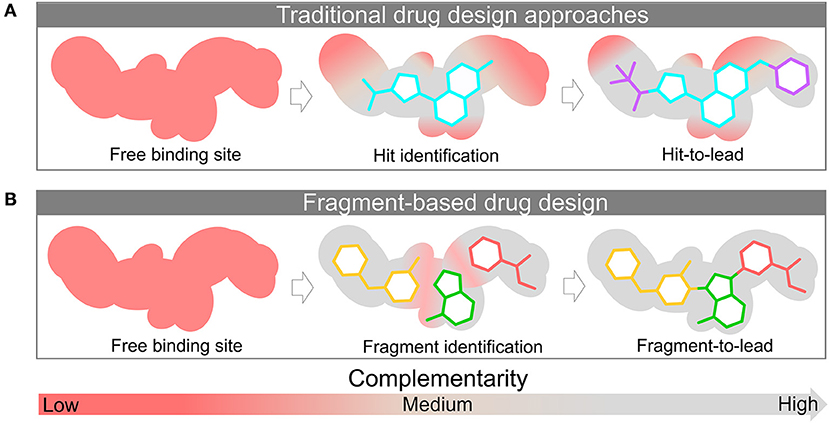
\includegraphics[width=\linewidth]{Chapters/Fresco/Figs/fbdd_vs_trad.jpg}
% \caption{An illustration comparing fragment-based drug discovery to traditional approaches.}
% \label{fig:fbdd}
% \end{figure}

Recently, advances in X-ray crystallography such as automatic crystal mounting robots, fast detectors, as well as increased accessibility to beamtime are enabling high throughput fragment screens. One can routinely go from screening a small fragment library and detecting a handful of hits, to screening 1000s of fragments with ensembles of 100s of fragments hits spanning the binding site \cite{Schiebel2016HighThroughput, Douangamath2020XChem}. This substantial increase in data enables a systematic data-driven approach for fragment-based hit discovery. 

% Although there exist some computational approaches for supporting FBDD, for example, hot spot analysis and pocket druggability prediction \cite{deSouza2020InSilicoFBDD}, at present, the main procedure of selecting which fragments to merge and how to do so remains largely intuition-based and human-driven.

% Follow-up compounds are then designed using chemical intuitions to merge spatially proximal fragments, or expand a fragment into promising binding pockets \cite{Ichihara2011FragLinking, Yu2021FragLinkingEntropy}. 

%Factoring in the rise of cryo-EM techniques as well \cite{Renaud2018CryoEMReview, Callaway2020RevolutionaryCryoEM}, we are reaching the stage where the data output will outpace traditional approaches for hit detection via FBDD. Let us consider the standard method of merging or linking pairs of fragments: given $N$ fragment hits, there are $\frac{N(N-1)}{2}$ possible choices of fragment pairs that could be combined. This means that if a fragment screen returns 100 hits, 4950 fragment pairs have to be considered, and for each of these pairs there are many possible ways to merge/link them into a potential hit compound.

%How to select a particular pair from these options, as well as how to perform the merging/linking of these fragments, remains largely intuition-based and human-driven \cite{Ichihara2011FragLinking, Yu2021FragLinkingEntropy}. Of course, not all of these possible pairings are chemically reasonable, but the overall quadratic scaling points to a growing headache where fragment screens give too many options to choose from, where increased data raises more questions than answers.

%When data throughput outstrips manual expertise, machine learning (ML) may provide the solution. By taking advantage of underlying patterns in large datasets, ML methods have recently provided breakthroughs in scientific domains such as protein-folding, chemical reaction prediction, and improving functionals in density functional theory. In the context of FBDD, ideally, we would like to use machine learning to leverage all of the available crystal structure data to inform our decision-making when advancing from a fragment screen toward hit detection. However, how to do so conceptually in terms of data featurization or model design has to the authors' knowledge never been discussed, let alone experimentally validated for hit detection.

Our key insight is to reframe fragment-based drug design as signal extraction from noisy data by seeking persistent pharmacophore correlations within a fragment ensemble, rather than looking at individual fragments. This is because a fragment itself has low affinity, thus we need the presence of multiple fragments with the same pharmacophore at a particular region of the binding site to provide statistical confidence. 

In this chapter, we employ unsupervised machine learning to learn the spatial distribution of fragment pharmacophores in the binding site. We then use the trained model as a scoring function for virtual screening, picking out molecules with matching pharmacophores. We will first retrospectively validate our model on a dataset of SARS-CoV-2 main protease (Mpro) ligands from COVID Moonshot \cite{Moonshot2022}. We then present prospective results on identifying hits against Mpro and the Mac1 domain of SARS-CoV-2 non-structural protein 3 (nsp3-Mac1) by performing a virtual screen of a library of 1.4 billion purchasable compounds from EnamineREAL.

% The only comparable methods that the authors are aware of are recent work in using deep generative models for proposing merges between two fragments (DeLinker \cite{Imrie2020DeLinker}, SyntaLinker \cite{Yang2020SyntaLinker}, and Develop \cite{Imrie2021Develop}). These approaches differ from ours in several ways: Firstly, these models all require human intervention from an expert in choosing which fragments to merge, or what pharmacophoric constraints need to be obeyed, whereas our model is fully end-to-end. Secondly, these methods utilise neural network-based generative models which are very sensitive to training hyperparameter choice in general (citation about mode collapse \cite{?}), and for molecular generation in particular, known to propose invalid and/or unsynthesizable molecules \cite{Gao2020Synthesizability}. In contrast, our method relies on kernel density estimation which is simple, robust, and free from hyperparameter tuning, and we explicitly only screen purchasable, easily-synthesised molecules. Lastly, the proposed models have only been studied computationally and lack validation in the real world.

% Our results are the first experimentally validated demonstration of hit detection via a fully computational workflow starting directly from an experimental fragment screen. This work opens the door for bridging fragment-based drug discovery with virtual screening.
\begin{figure}[!bh]
 \centering
 \begin{subfigure}{\textwidth}
 \centering
 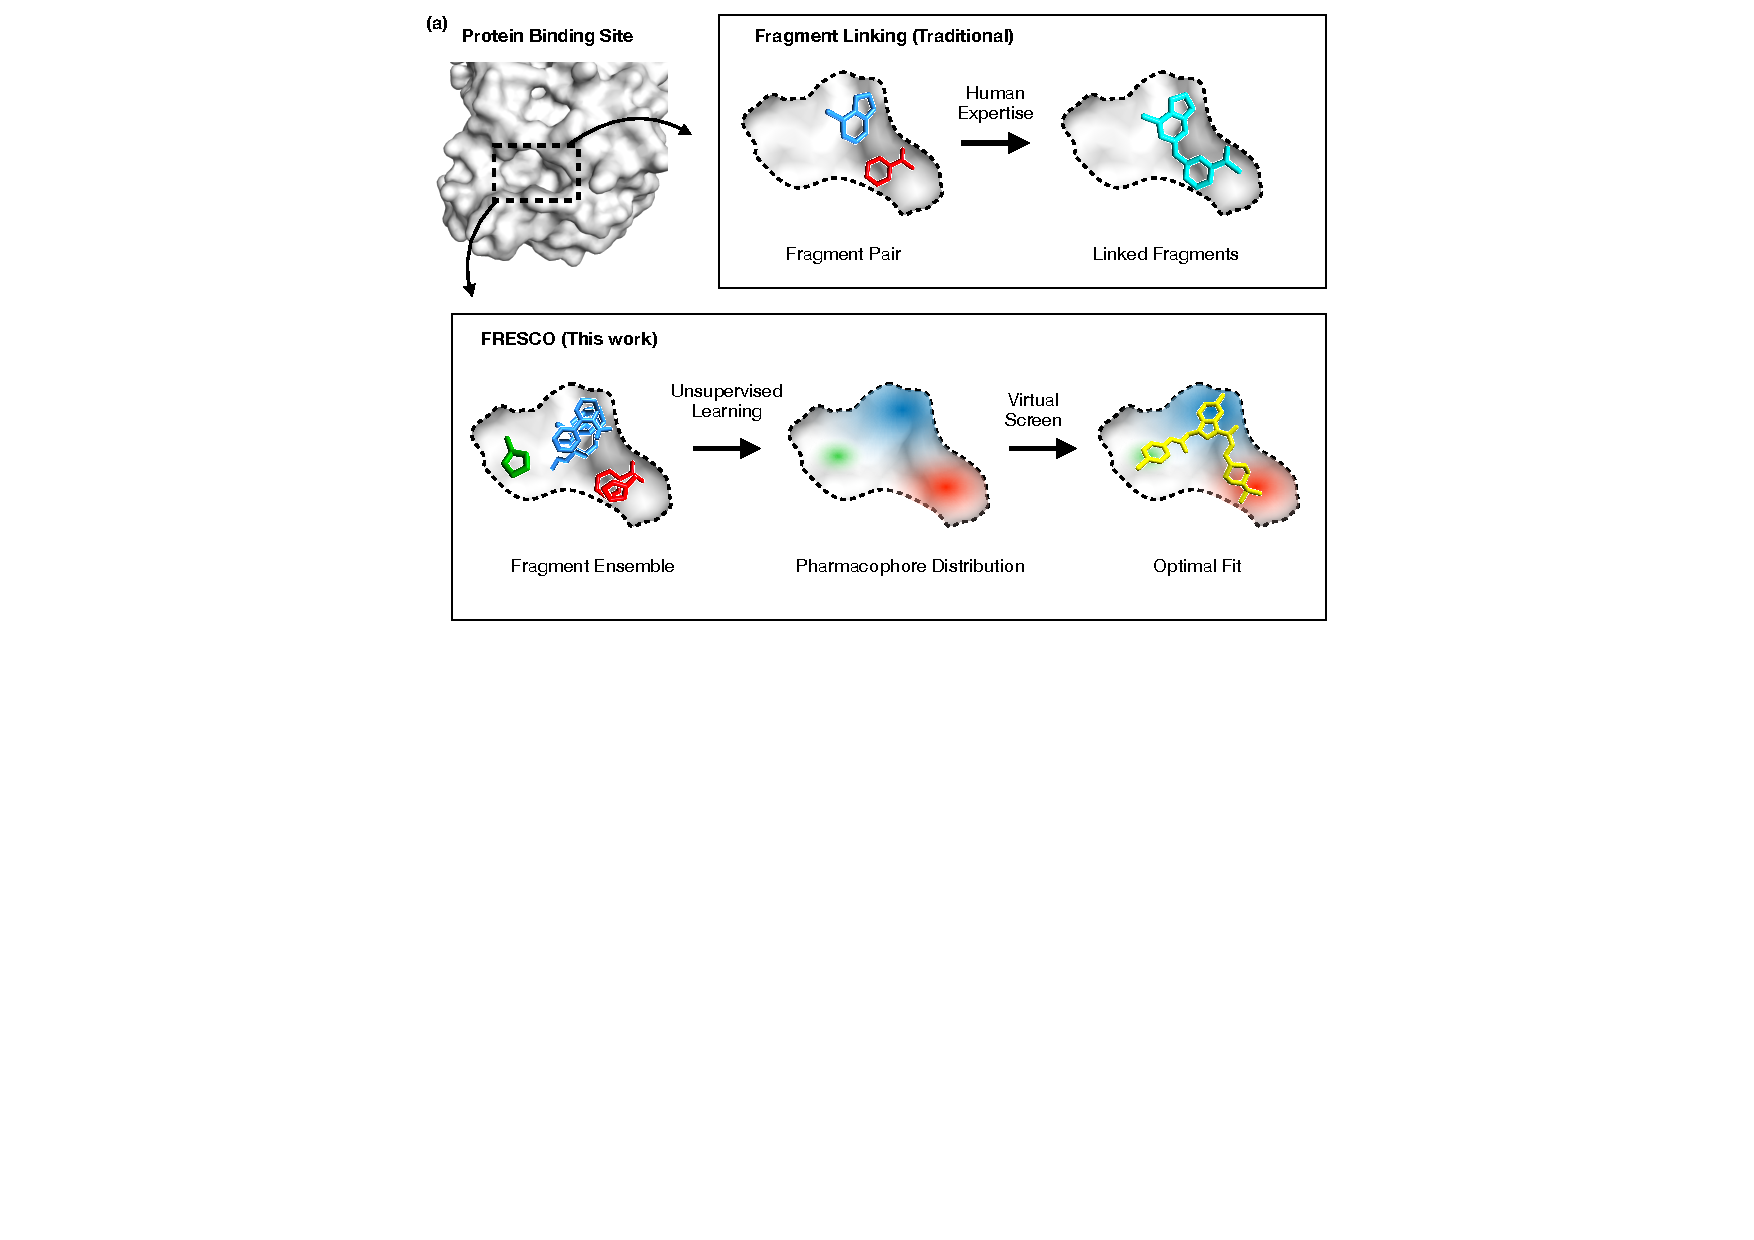
\includegraphics[width=0.75\textwidth]{Chapters/Fresco/Figs/fresco_vs_linking_a.pdf}
 
 \end{subfigure}
 \hfill
 \begin{subfigure}{\textwidth}
 \centering
 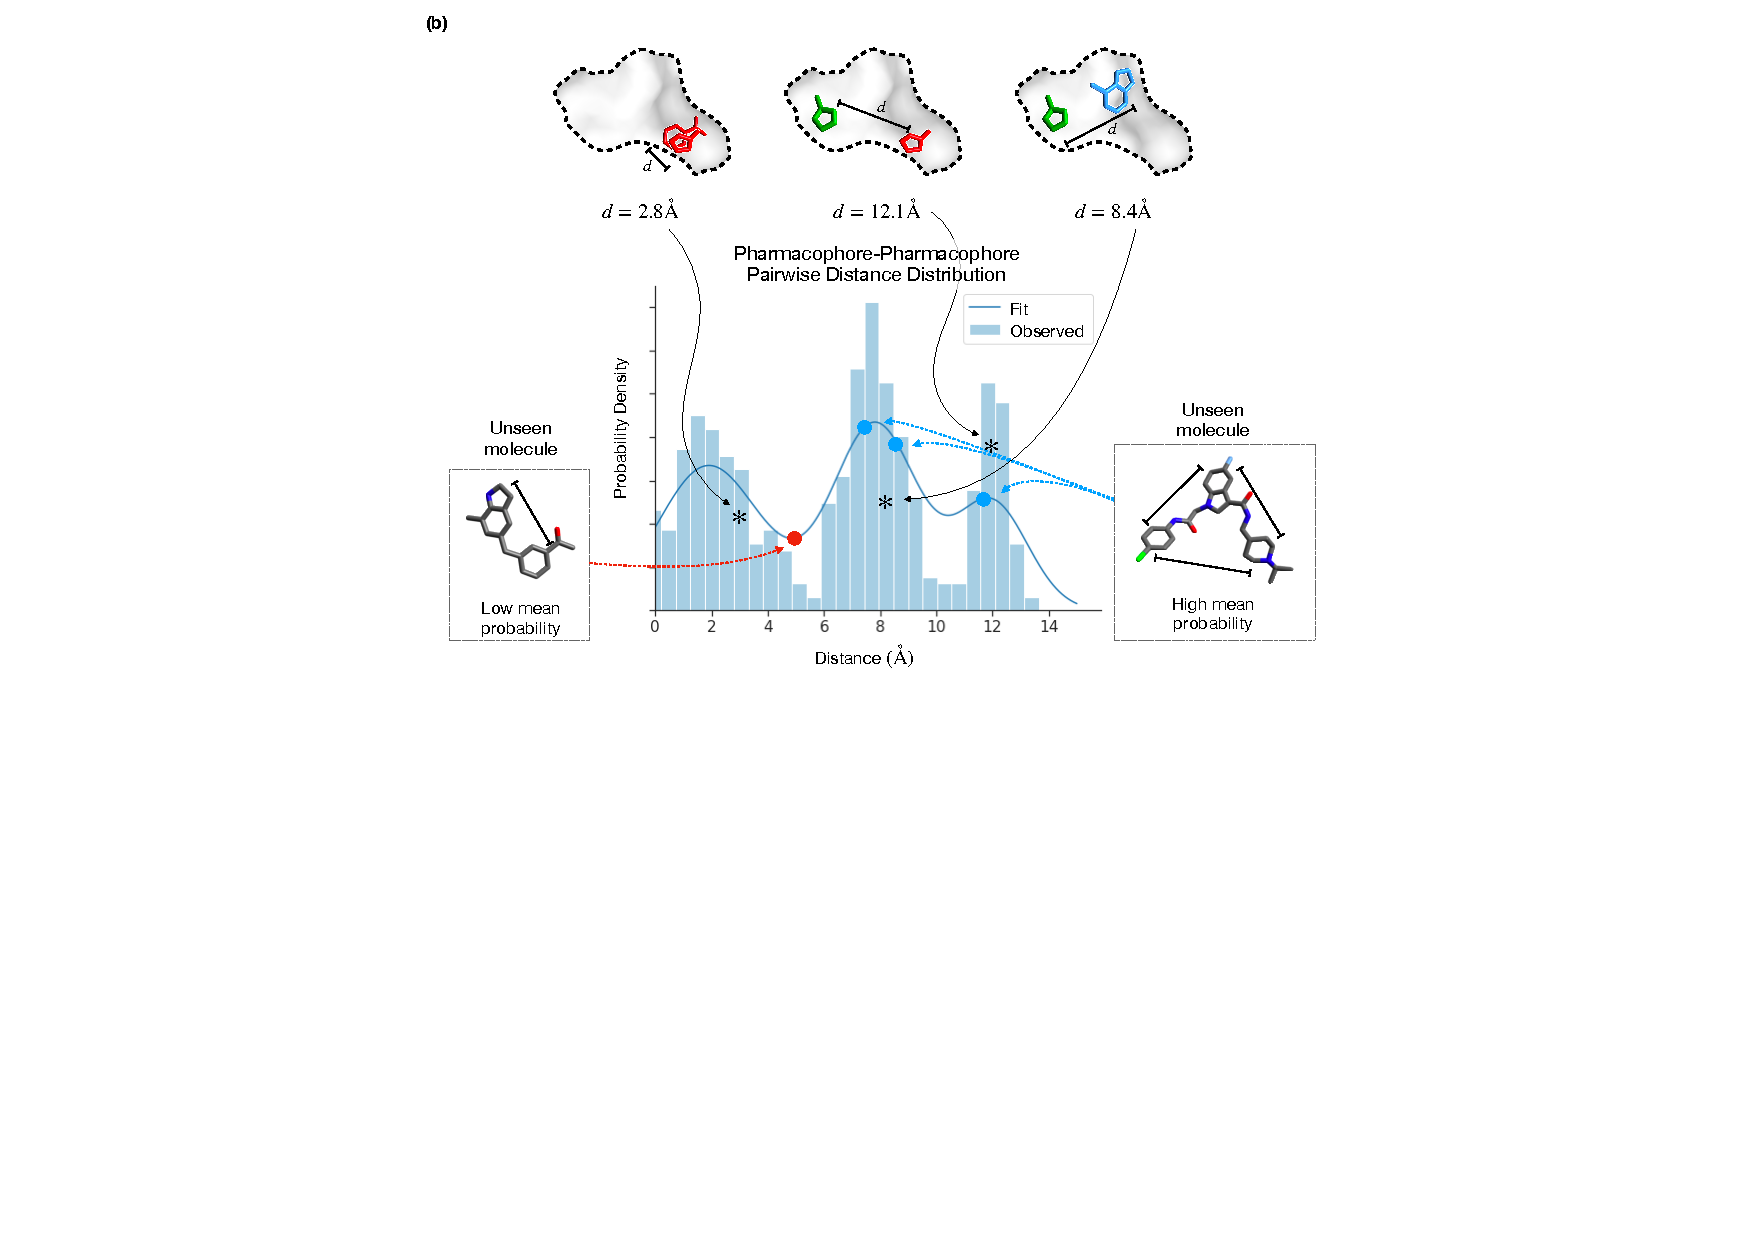
\includegraphics[width=0.75\textwidth]{Chapters/Fresco/Figs/fresco_details.pdf}

 \end{subfigure}
 \caption{\textbf{Illustrations of the FRESCO method.} (\textbf{a}) FRESCO conceptually differs from traditional fragment merging/linking by taking a distributional approach. (\textbf{b}) Unsupervised learning of the distribution of pairwise pharmacophore distances from fragment ensembles allows the virtual screening of unseen molecules.}
 \label{fig:fresco_vs_linking}
\end{figure}

\section{Unsupervised Learning of Pharmacophore Distributions} \label{sec:model}

\begin{figure}[th]
 \centering
 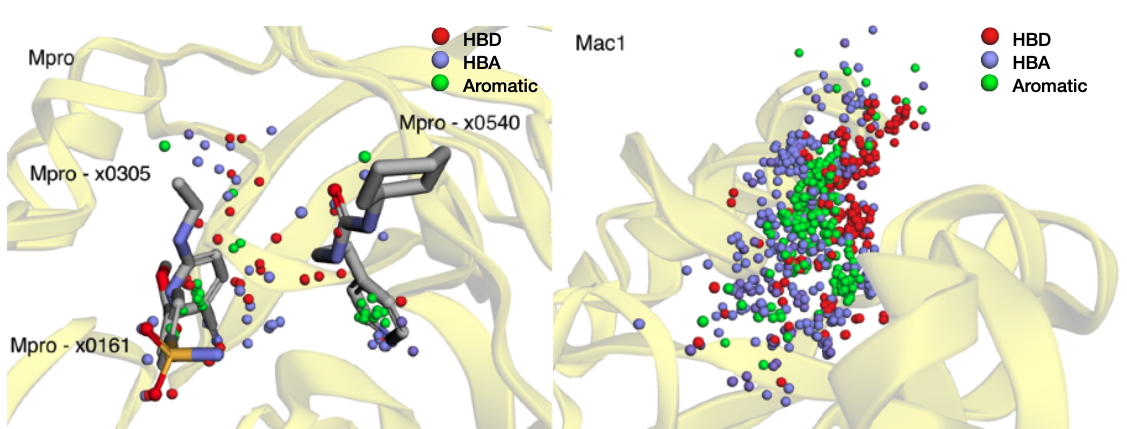
\includegraphics[width=0.8\textwidth]{Chapters/Fresco/Figs/pharmacophores.png}
 \caption{\textbf{Examples of pharmacophore distributions from fragment ensembles.} The red, blue, and green spheres depict hydrogen bond donors, acceptors, and aromatic pharmacophores respectively from fragment ensembles in the 3D binding sites of (\textbf{a}) Mpro, and (\textbf{b}) nsp3-Mac1. Several of the Mpro fragments are drawn to illustrate the ‘origin’ of some pharmacophores. None are drawn for nsp3-Mac1 due to the density of pharmacophores in the binding site.}
 \label{fig:pharmacophores}
\end{figure}


To turn fragment hits into a model that predicts whether an unknown ligand will bind potently to the binding site, we employ an interpretation inspired by statistical physics. There are multiple chemical motifs that can engage residues on the binding site. These different modes of engagement can be considered as a statistical distribution. Each interaction between a chemical motif on the fragment and a binding site residue corresponds to an instance of this statistical distribution. We assume that the fragment library broadly covers chemical space, and anticipate that stronger interactions will be sampled and therefore observed more often amongst fragment hits than weaker interactions. Note that an individual fragment is a weak binder -- fragment screens are done at a high concentration which forces the equilibrium towards forming fragment-protein complexes enabling detection via crystallography. Therefore, we analyse the statistical distribution of fragment-protein interactions formed by the dense fragment hits, rather than any individual fragment (Figure \ref{fig:fresco_vs_linking}a).

To numerically approximate this distribution, we quantify binding interactions by coarse-graining the fragment molecules into hydrogen-bond donor, hydrogen-bond acceptor, and aromatic ring ``pharmacophores'' (Figure \ref{fig:pharmacophores}). These are simple abstractions of molecular features that can make potent interactions with binding site residues and is a commonly used tool to interpret the biological activity of ligands \cite{Kaserer2015PharmacophoreReview}. The distribution which we then choose to approximate is the pair-wise distance between these pharmacophores. Computational screening of compounds based on pharmacophore distances is a commonly used technique in medicinal chemistry, though here we are extending this concept to enable a statistical interpretation of fragment hit. We consider pharmacophore features, rather than specific protein-ligand interactions so that the downstream model takes the ligand as the input rather than having to perform the additional step of computationally placing the ligand in the binding site. 

%in fragment-based hit dis intention of replicating the intuition of a medicinal chemist deducing spatial correlations between pharmacophores from different fragments.

We utilise kernel density estimation (KDE) \cite{Parzen1962KDE} to estimate this spatial distribution of pair-wise pharmacophore distances. We then score unseen molecules by evaluating pharmacophore distances within that molecule against the probability distribution of pharmacophore distances derived from the fragment ensemble (Figure \ref{fig:fresco_vs_linking}b). We take the mean probability over all of the distances between all possible pharmacophore-pharmacophore pairs as the score for the molecule. This is an unsupervised approach -- starting from the results of a crystallographic fragment screen, without any bioactivity data, we can build a model that computationally screens unseen molecules. We term our approach Fragment Ensemble Scoring (FRESCO). 

FRESCO conceptually departs from machine learning approaches in the literature for fragment-based hit discovery. These approaches, such as DeLinker \cite{Imrie2020DeLinker}, SyntaLinker \cite{Yang2020SyntaLinker}, and Develop \cite{Imrie2021Develop}), as well as data-mining methods such as Fragment Network \cite{Hall2017FragNet}, attempt to grow single fragments or merge only a pair of fragments. They all require expert insights in choosing which fragments to merge, or what pharmacophoric constraints need to be obeyed, instead of leveraging all of the information from an ensemble of fragment hits in a data-driven manner.

FRESCO also closes a gap in the burgeoning literature on machine learning for bioactivity prediction \cite{muratov2020qsar}. These models cannot be used when no training data exists, as is the case in the hit-finding phase. Thus a new modelling approach -- here we employed unsupervised learning -- is needed to tackle the ``zero-to-one'' problem. Although physics-based models of ligand-protein binding such as docking \cite{Lyu2019UltraLargeDocking, Alon2021sigma, Fink2022Alpha} can be used in the absence of any bioactivity data, FRESCO crucially incorporates information from the fragment screen on preferential interactions between regions of the binding site and the fragment pharmacophores.

We validate our approach by performing a retrospective study on historical data, as well as embarking on prospective campaigns on two different protein targets. Retrospective tests or benchmarks, typically the only method used to compare machine learning models, are insufficient for measuring the impact of incorporating the model in the decision-making process of compound selection in drug discovery \cite{Kearnes2021Prospective}. Thus we go beyond typical model development and undertake a prospective search for hit molecules using only FRESCO to obtain a more realistic measure of its performance.

\subsection{Model Implementation} \label{subsec:model_construction}

To train our model, we first process a set of experimental fragment-protein complexes. In this particular work, we downloaded structures from the \href{https://fragalysis.diamond.ac.uk/viewer/react/landing}{\texttt{Fragalysis}} platform \cite{Douangamath2020XChem}. For Mpro, non-covalent fragments from the XChem fragment screen \cite{Douangamath2020XChem} were used while for Mac1 both XChem and UCSF fragment data were used \cite{Schuller2021Mac1Frag}.

We then extract the pharmacophore features from the fragment molecules and their corresponding conformer coordinates. Specifically, we used SMARTS pattern matching following default pharmacophore definitions in \href{https://www.rdkit.org/docs/index.html}{\texttt{RDKit}} \cite{rdkit} to extract pharmacophores from the fragment SMILES. The pharmacophores considered are hydrogen bond donors, hydrogen bond acceptors, and aromatic rings. The corresponding coordinates for each pharmacophore are defined as the average over the atoms in the pharmacophore (eg the position of an aromatic pharmacophore from a benzene ring would be the mean of the coordinates of the 6 carbon atoms in the ring). We then compute the matrix of pairwise distances between all possible pharmacophore pairs (eg Donor-Donor \& Aromatic-Acceptor) between different fragment molecules. The flattened distance matrix for each pharmacophore pair is the distribution that we choose to model.

For some fragments, multiple crystallographic poses are recorded. To account for this, we weigh the contribution of each fragment structure to the overall fragment pharmacophore distribution by $\frac{1}{n}$ where $n$ is the number of conformations recorded for each conformer. In addition, we exclude the counting of correlations between pharmacophores from the same fragment - only correlations between different fragments are measured. This is to avoid spurious intra-fragment correlations that are unrelated to binding to the binding site - strong correlations in pharmacophore distribution between multiple independent fragments are indicative of useful binding interactions and these are what we hope to capture with this methodology.

With the processed 3D pharmacophore distributions, we can then fit a FRESCO model by learning the probability distribution of the pairwise distances using kernel density estimation (KDE). The bandwidth for KDE fitting was chosen for each pairwise distribution using the Improved Sheather-Jones algorithm \cite{Botev2010ISJ}. Each pharmacophore pair is associated with its own KDE, and the collection of KDE models for all of the pharmacophore pairs comprises the FRESCO model.

With a trained FRESCO model, we can then score unseen molecules by evaluating the probability of the pharmacophore distribution of each molecule. Given a set of input molecular conformers (eg from docking), the same processing workflow is used to obtain the 3D pharmacophore distributions of each molecule, and the probabilities of each distribution are evaluated using the KDEs. The overall score for the molecule is returned as the mean log-probability over all of the pairwise pharmacophore combinations.

\section{Computational Retrospective Study} \label{sec:retrospective}

To validate FRESCO, we evaluate how our method compares against the computational approach of docking, as well as the human expertise of medicinal chemists. Specifically, we wish to estimate the extent to which FRESCO could have accelerated hit identification in a fragment-based drug discovery campaign. This requires a dataset that is explicitly exhibiting structure-activity data from the fragment-to-lead phase of a campaign to accurately reflect the degree of structural diversity and distribution of molecular activity. The use of data from an early-stage high-throughput screen would exaggerate the diversity of structures explored, while data from the lead-optimisation phase of a campaign would artificially contain many potent molecules.

For this reason, we choose to study the COVID Moonshot campaign \cite{Moonshot2022} which is targeting the SARS-CoV-2 main protease (Mpro). COVID Moonshot is, to our knowledge, the only openly available dataset of fragment-to-lead drug discovery, driven by a community of medicinal chemists, where every structure and associated activity is disclosed. This unique dataset allows us to perform a time-split analysis, focusing on the fragment-to-lead phase (see Section \ref{sec:background_moonshot} for more details on COVID Moonshot).

The Moonshot activity data for the retrospective study was accessed on Mar 22nd, 2021. The IC50 values in that dataset, as well as in the prospective study on Mpro were measured from a fluorescence-based enzyme activity assay, the details of which are described below. To narrow down the data to molecules during the fragment-to-lead stage of the Moonshot campaign, we only selected molecules that were designed before September 1st, 2020, which gave us a dataset of 979 compounds.

In addition, molecular docking studies have also been done extensively on molecules from the Moonshot campaign \cite{Morris2021Rank, Saar2021biorxiv}. For our analysis we utilise the same docking protocols as those reported previously for consistency, the details of which can be found in the methods section.

In the hit identification phase of drug discovery, relatively little is known about what ligand-protein interactions are feasible, thus most proposed molecules are unlikely to be active. A meaningful metric for comparing methods in this regime is the top-$N$ ``hit rate'', which measures the percentage of the top-$N$ predictions which are active. We expect the curve from plotting the hit rate against $N$ of an informative method to be consistently higher than that of a less informative method. For the Moonshot data, we set an IC50 (concentration of inhibitor required to inhibit 50\% of protein activity) threshold of 5\uM for defining a ``hit''.

The baseline hit rate in the dataset i.e. the percentage of compounds with IC50 $<$ 5\uM, is 6.0\%. This represents the hit rate of medicinal chemists using traditional and computational tools at their disposal to design compounds for the Moonshot drug discovery campaign. The hit rate for docking is computed by choosing the top-$N$ molecules with the best score. To calculate the hit rate for FRESCO, we first fit a FRESCO model on 23 publicly reported crystallographic structures of non-covalent fragments bound to the SARS-CoV-2 Mpro protein \cite{Douangamath2020XChem} and score the whole dataset using the fitted FRESCO model.

% \begin{figure}[th]
%  \centering
%  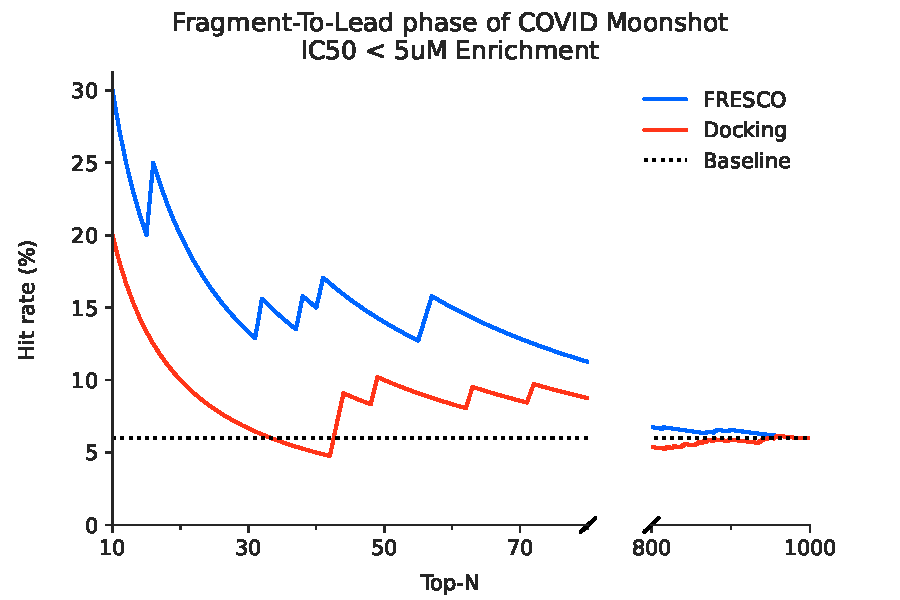
\includegraphics[width=0.8\textwidth]{Chapters/Fresco/Figs/fresco_vs_moonshot_break_5uM.pdf}
%  \caption{\textbf{FRESCO is able to retrospectively perform hit detection.} High hit rates are achieved relative to docking and the human expert baseline when ranking molecules from the fragment-to-lead phase of COVID Moonshot.}
%  \label{fig:moonshot_enrichment_vs_docking}
% \end{figure}

\begin{figure}[!th]
    \centering
   
    \begin{subfigure}{\textwidth}
    \centering
    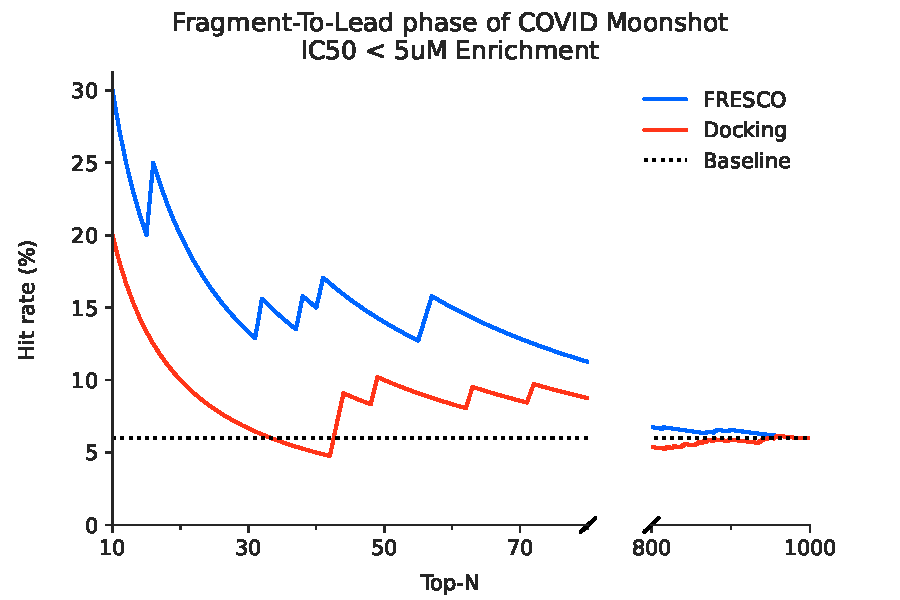
\includegraphics[width=0.8\textwidth]{Chapters/Fresco/Figs/fresco_vs_moonshot_break_5uM.pdf}
    \end{subfigure}
    \hfill
   
    \begin{subfigure}{\textwidth}
    \centering
    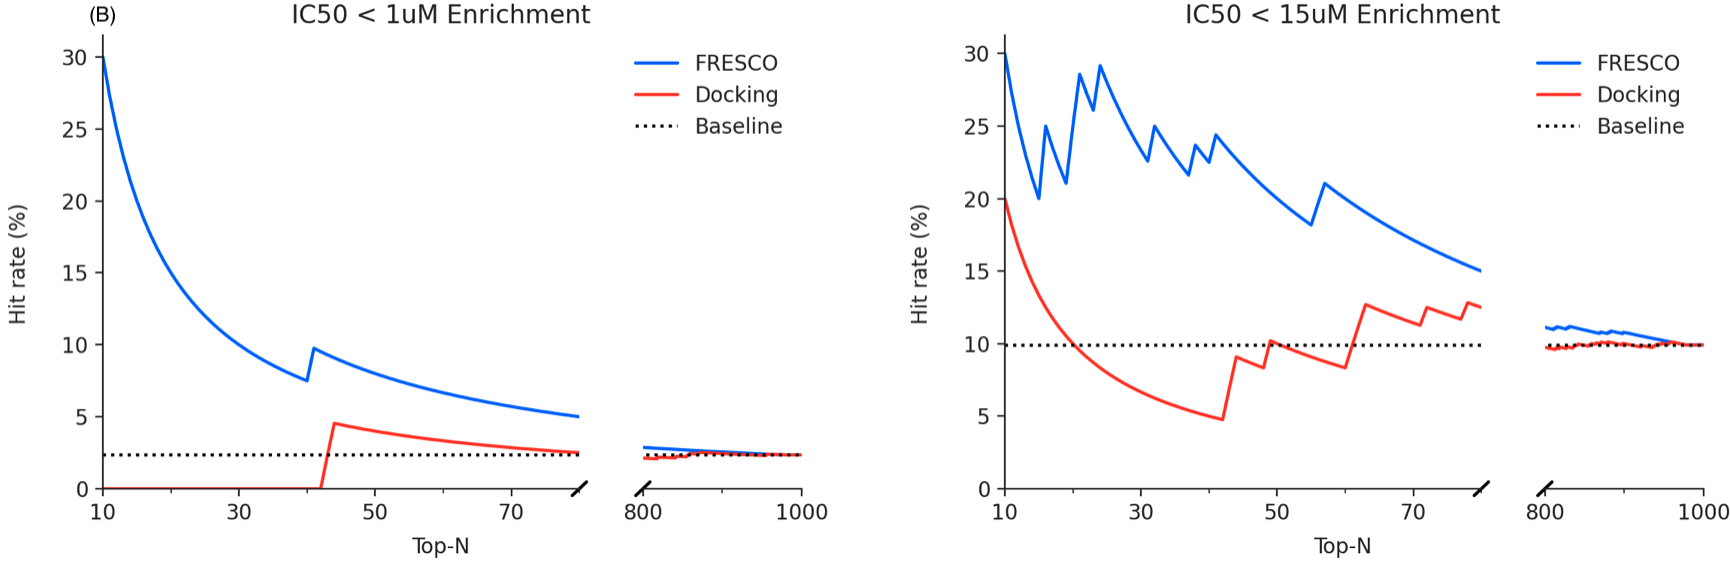
\includegraphics[width=1.0\textwidth]{Chapters/Fresco/Figs/fresco_sensitivity.png}
    \end{subfigure}
    \caption{\textbf{FRESCO is able to retrospectively perform hit detection.} High hit rates are achieved relative to docking and the human expert baseline when ranking molecules from the fragment-to-lead phase of COVID Moonshot.}
    \label{fig:moonshot_enrichment_vs_docking}
\end{figure}

Figure \ref{fig:moonshot_enrichment_vs_docking} shows that FRESCO achieves higher hit rates compared to both computational docking and medicinal chemists. Looking at the top-5\% of the molecules ($N<50$), FRESCO has a hit rate of 12-30\%, roughly 2-5 times that of the medicinal chemists. The threshold for defining a hit compound is relatively arbitrary and repeated analysis for both lower and higher IC50 thresholds (1-15\uM) show similar results (Figure \ref{fig:moonshot_enrichment_vs_docking}B). This shows that it is possible to correlate bioactivity with unsupervised learning of fragment pharmacophore distributions and that FRESCO could accelerate hit detection in a real-world drug discovery campaign. In this retrospective study, FRESCO is standing on the shoulders of medicinal chemists -- it is used to re-score compounds that are designed by chemists. Therefore, we next turn to interrogate the performance of FRESCO in a real-world context when it is used to score a large unbiased library of compounds via a series of prospective studies. 


\begin{figure}[!h]
 \centering
 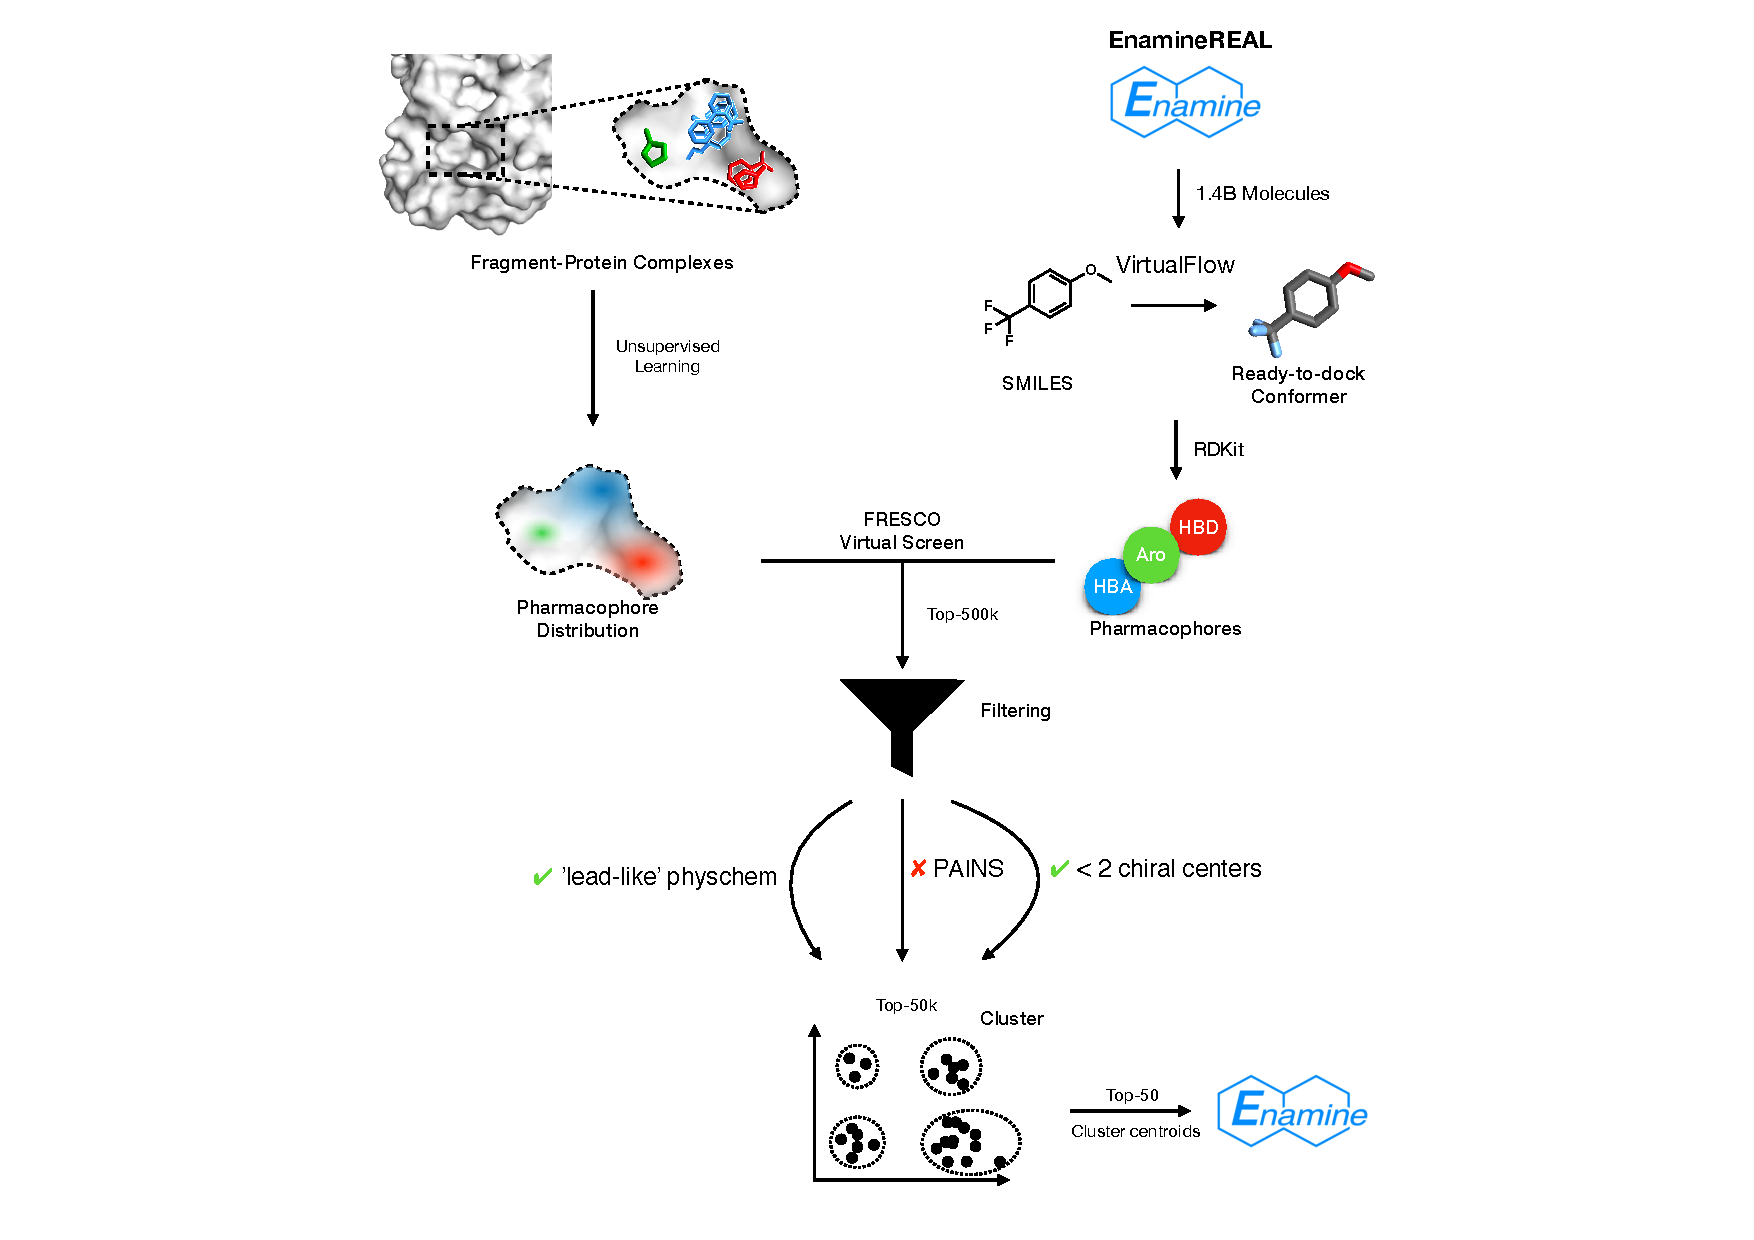
\includegraphics[width=\linewidth]{Chapters/Fresco/Figs/flowchart_details.pdf}
 \caption{\textbf{A schematic of the FRESCO screening workflow.} Target-specific FRESCO models are applied on pre-processed conformers of compounds from EnamineREAL to score them. The top-ranked compounds are then filtered by their physical properties, and clustered by structural similarity. Diverse compounds are chosen for synthesis by picking centroids of the most populous clusters.}
 \label{fig:screening_workflow}
\end{figure}

\section{Prospective hit finding} \label{sec:prospective}

Building on the results of the retrospective evaluation, we performed a prospective study on Mpro. Rather than rescreening Moonshot compounds, we instead deploy the model to virtually screen a library of commercially available compounds. By synthesising and assaying the top-ranked compounds, we can evaluate the performance of FRESCO in a real-life use case of hit discovery.

The computational workflow we follow to perform the virtual screening is shown in Figure \ref{fig:screening_workflow}. Using a FRESCO model trained on the fragment-protein complexes, we score the library and rank the compounds by score. The top-ranked compounds are then filtered by their physical properties to maximise ``drug-likeness'', and selected diverse compounds by clustered hit by structural similarity and picking centroids of the most populous clusters.

The library we screen is VirtualFlow, a published dataset of more than 1.4 billion commercially available molecules from EnamineREAL \& ZINC15 with pre-generated molecular conformers in a ready-to-dock format \cite{Gorgulla2020VirtualFlow}. The top-500k predictions were selected and filtered to remove undesirable properties. A series of successive filtering steps were performed: first, only molecules with physical properties in well-understood ``lead-like'' chemical space \cite{ChemSpace} were kept. Then, we remove molecules that match known filters for pan-assay interference compounds (PAINS) \cite{Baell2010Pains} as well as filters for moieties that are undesirable for medicinal chemistry (eg furan, thiophene, nitro groups). Duplicate tautomers for each molecule are also removed. Finally, for ease of synthetic accessibility, we only consider molecules with less than two chiral centers.

The top-50k molecules remaining from the filtering were then clustered via Butina Clustering \cite{Butina1999Clustering} with a Tanimoto distance threshold of 0.2. This resulted in 24748 for Mpro. The centroids of the 50 most populous clusters (or the closest purchasable analogue if it wasn't available) were chosen as the candidate compounds. These compounds were ordered for synthesis from Enamine which resulted in 38 successfully made molecules.

% This resulted in 24748 and 22358 clusters for Mpro and Mac1, respectively. For both targets, the centroids of the 50 most populous clusters (or the closest purchasable analogue if it wasn't available) were chosen as the candidate compounds. These compounds were ordered for synthesis from Enamine which resulted in 38 and 52 successfully made molecules for Mpro and Mac1, respectively.

\begin{figure}[!ph]
 \centering

 \begin{subfigure}{\textwidth}
 \centering
 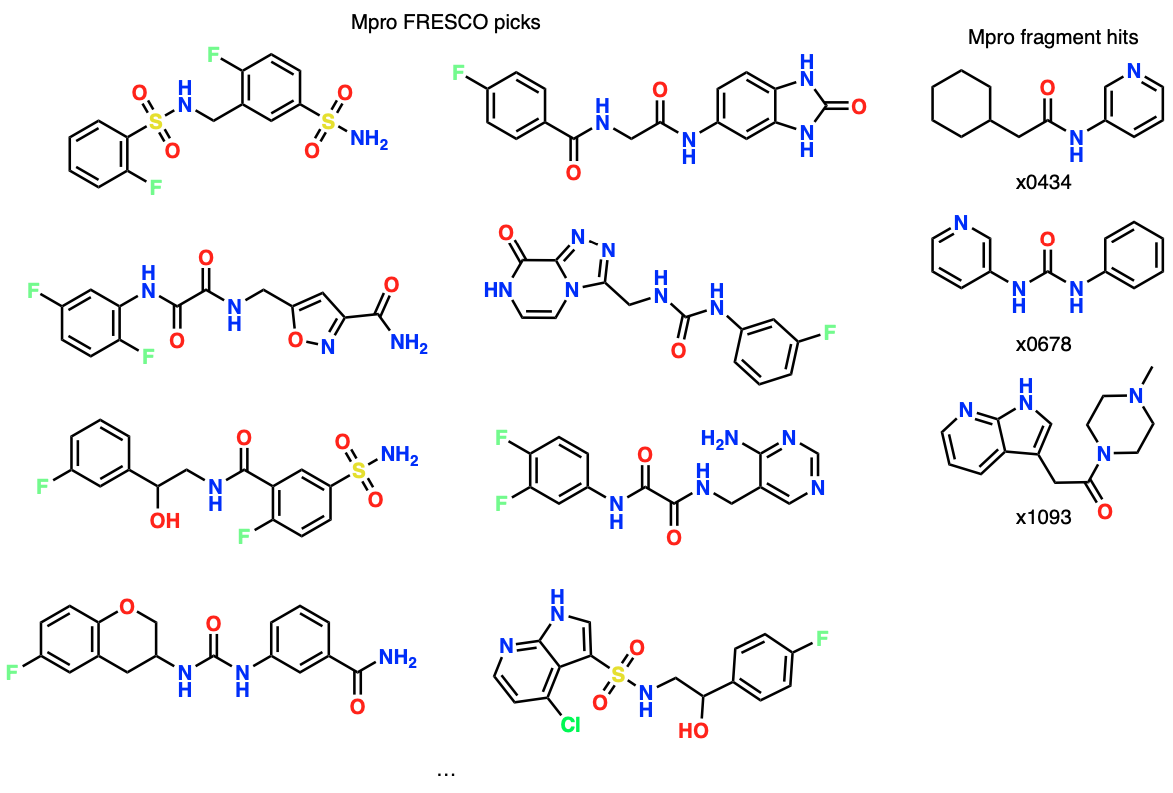
\includegraphics[width=0.75\linewidth]{Chapters/Fresco/Figs/mpro_ligands.png}
 % \caption{(a) Example structures of cluster centroids after executing the FRESCO screening workflow on Mpro. The molecules favoured by FRESCO tend to have 2 aromatic moieties connected via an amide or an amide isostere, similarly exhibited by three of the initial fragment hits whose structures are also shown.}
 % \label{fig:mpro_ligands}
 \end{subfigure}
 \hfill

 \begin{subfigure}{\textwidth}
 \centering
 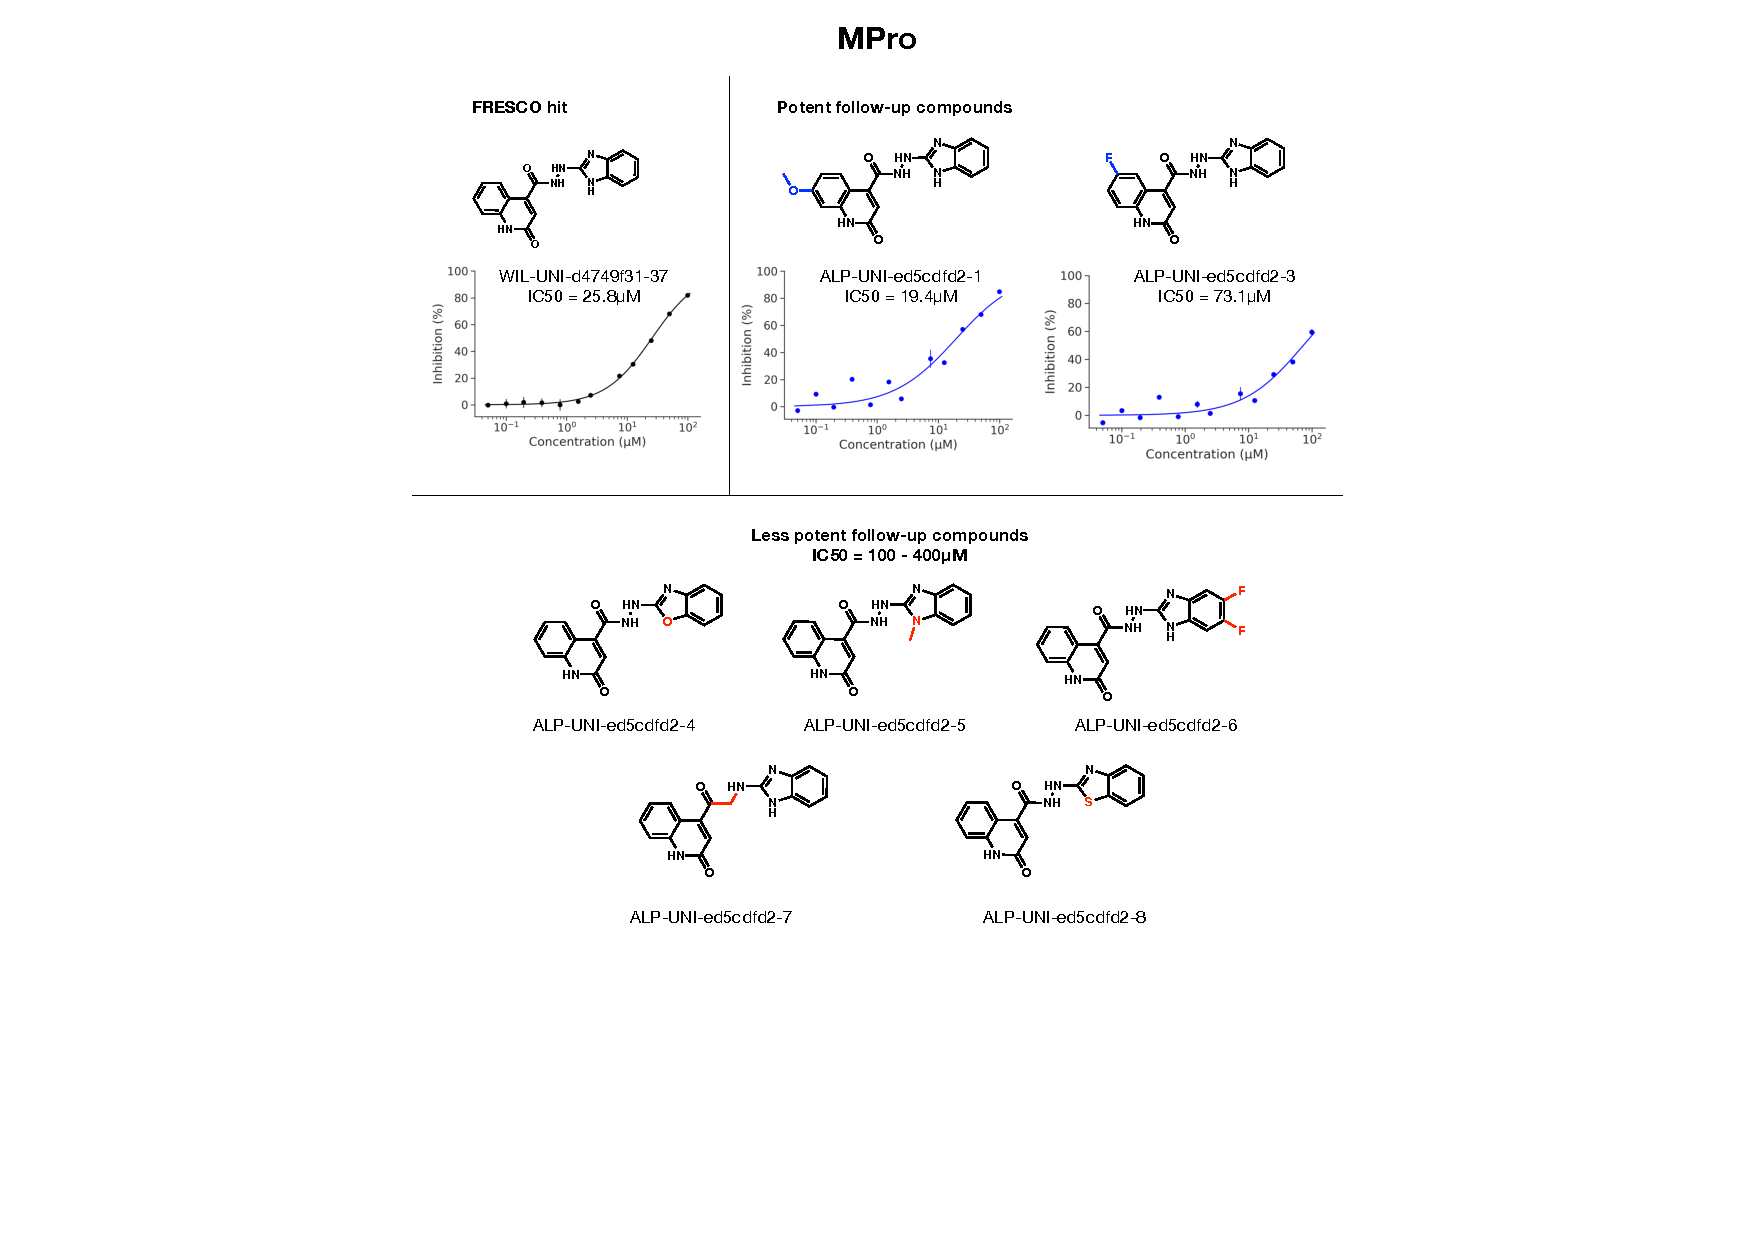
\includegraphics[width=0.75\linewidth]{Chapters/Fresco/Figs/mpro_hit_IC50.pdf}
 % \caption{Compound WIL-UNI-d4749f31-37 is identified as a hit against Mpro, with hit confirmation via follow-up compounds demonstrating SAR. Perturbations to the 2-hydroxyquinoline substructure of WIL-UNI-d4749f31-37 led to increased potency while changes to the benzimidazole group consistently decreased potency. Structural differences between the follow-up compounds and WIL-UNI-d4749f31-37 are highlighted in blue/red.}
 % \label{fig:mpro_hit}
 \end{subfigure}
 \caption{\textbf{FRESCO prospectively identifies a hit against Mpro.} (\textbf{a}) The molecules favoured by FRESCO tend to have 2 aromatic moieties connected via an amide or an amide isostere, similarly exhibited by three of the initial fragment hits whose structures are also shown. (\textbf{b}) Compound WIL-UNI-d4749f31-37 is identified as a hit against Mpro, with hit confirmation via follow-up compounds demonstrating SAR. Perturbations to the 2-hydroxyquinoline substructure of WIL-UNI-d4749f31-37 led to increased potency while changes to the benzimidazole group consistently decreased potency. Structural differences between the follow-up compounds and WIL-UNI-d4749f31-37 are highlighted in blue/red.}
 \label{fig:mpro_results}
\end{figure}

% \begin{figure}[!hbtp]
% \centering
% 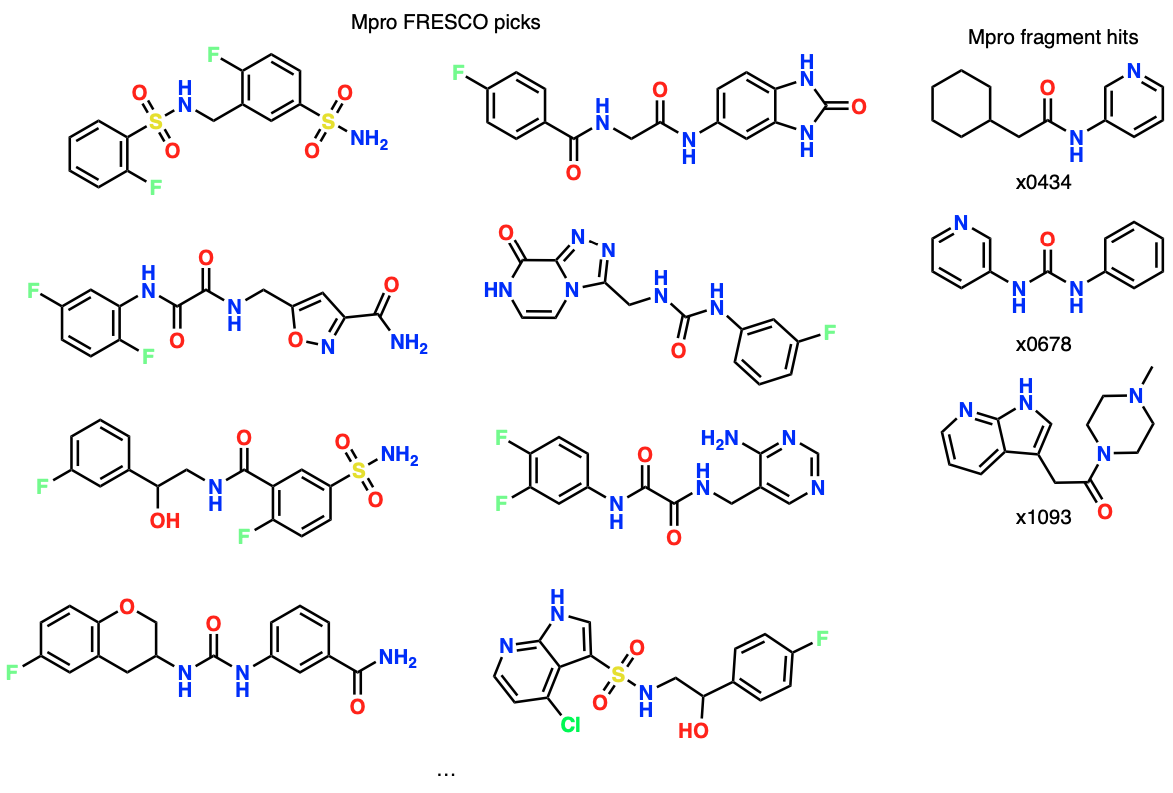
\includegraphics[width=0.75\linewidth]{Chapters/Fresco/Figs/mpro_ligands.png}
% \label{fig:mpro_ligands}
% \caption{Example structures of cluster centroids after executing the FRESCO screening workflow on Mpro. The molecules favoured by FRESCO tend to have 2 aromatic moieties connected via an amide or an amide isostere, similarly exhibited by three of the initial fragment hits whose structures are also shown.}
% \end{figure}

% \begin{figure}
% \centering
% 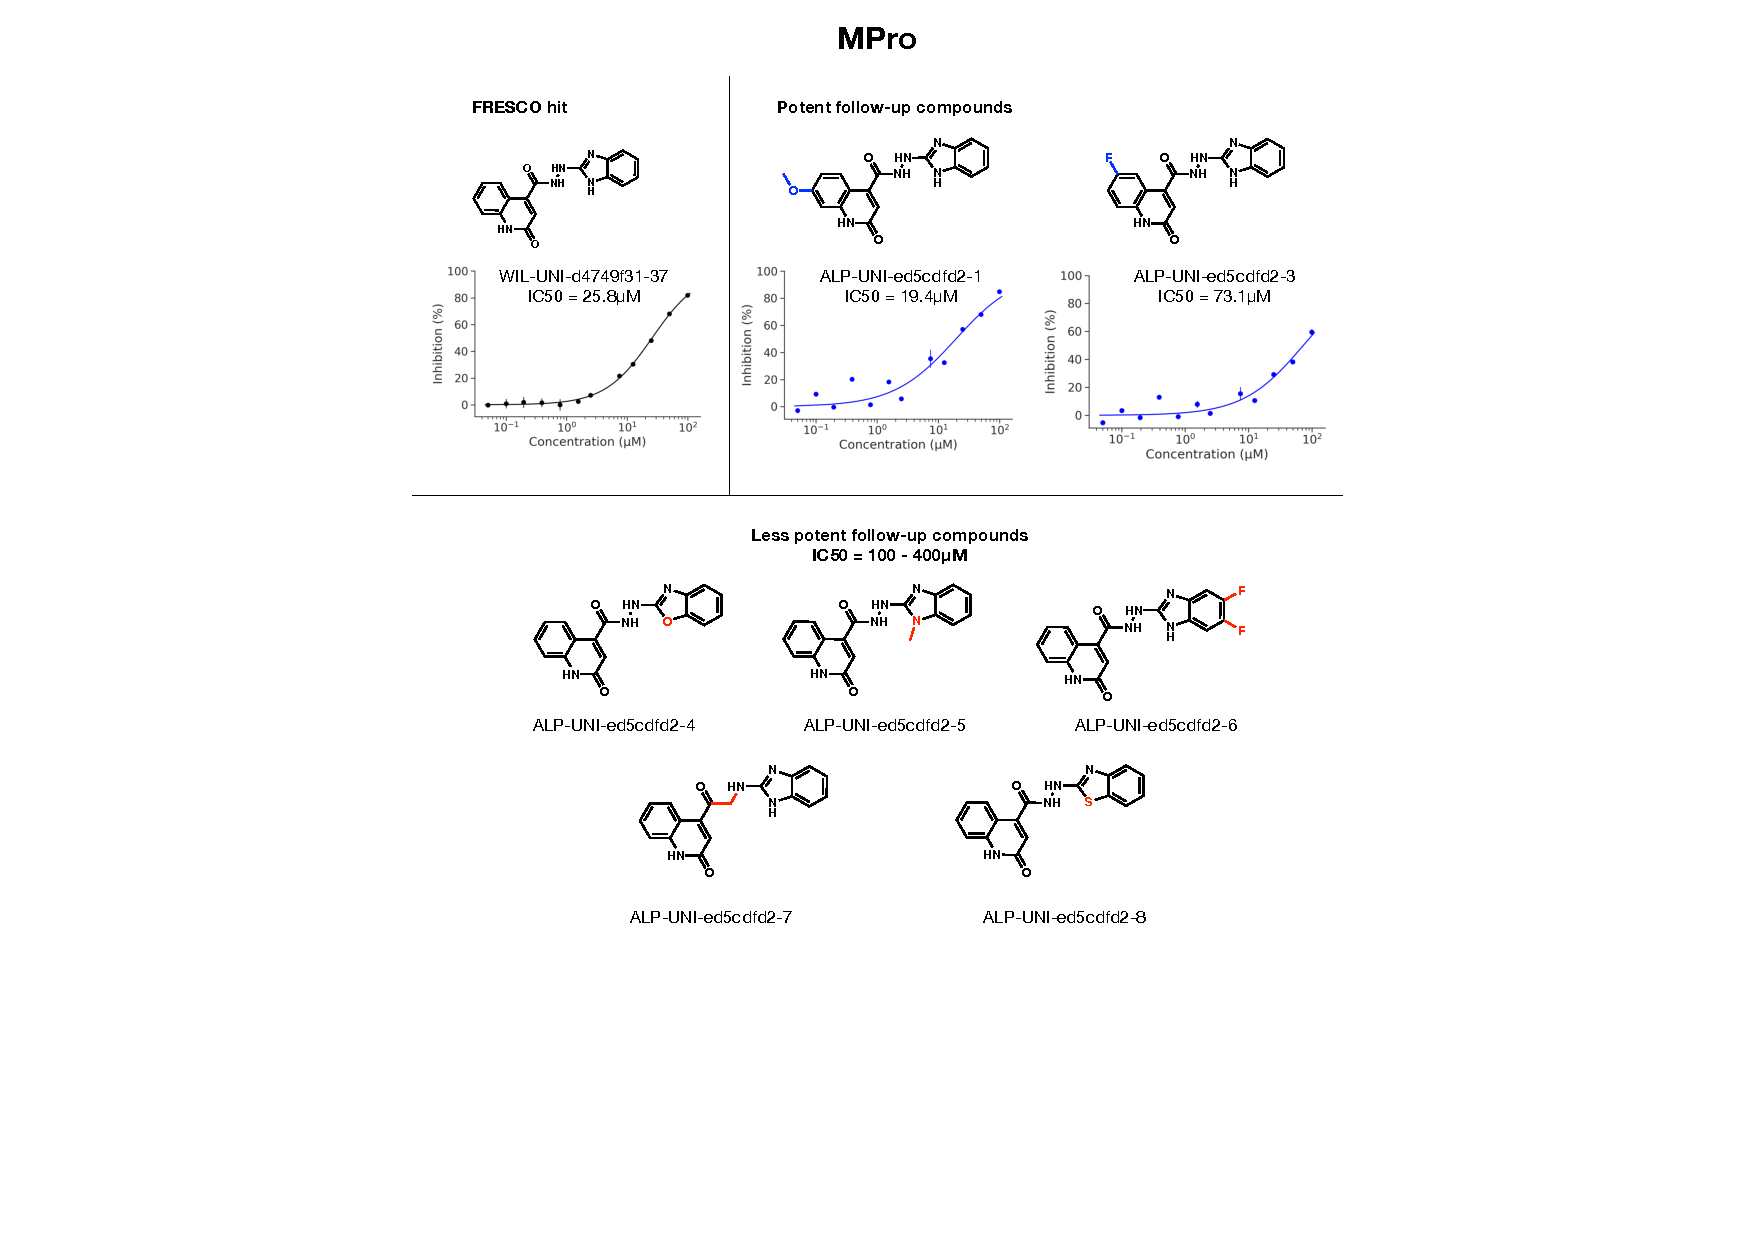
\includegraphics[width=0.75\linewidth]{Chapters/Fresco/Figs/mpro_hit_IC50.pdf}
% \label{fig:mpro_hit}
% \caption{Compound WIL-UNI-d4749f31-37 is identified as a hit against Mpro, with hit confirmation via follow-up compounds demonstrating SAR. Perturbations to the 2-hydroxyquinoline substructure of WIL-UNI-d4749f31-37 led to increased potency while changes to the benzimidazole group consistently decreased potency. Structural differences between the follow-up compounds and WIL-UNI-d4749f31-37 are highlighted in blue/red.}
% \end{figure}

Inspecting the cluster centroids favored by FRESCO, we observe typically 2 aromatic moieties connected via an amide or amide isostere. This scaffold is exhibited by three of the initial fragment hits (x0434, x0678, x1093), with most of the other fragment hits possessing an aromatic group bound at similar locations (Figure \ref{fig:mpro_results}a). The most promising compound, WIL-UNI-d4749f31-37, has an IC50 of 25.8\uM measured via fluorescence assay while the remaining compounds were found to be weak-to-negligible activity.

To validate compound activity, the COVID Moonshot Consoritium synthesized synthesized 8 close analogues to demonstrate the existence of responsive Structure-Activity Relationship \cite{Hermann2013ZincImpurity, Morreale2017ZincImpurity} (Figure \ref{fig:mpro_results}b). 3 of those compounds, which contained modifications to the 2-hydroxyquinoline substructure of WIL-UNI-d4749f31-37, retained relatively high potency of IC50 $<$ 100\uM with one of them (ALP-UNI-ed5cdfd2-1) exhibiting a lower IC50 of 19.4\uM. The remaining 5 compounds which perturbed the benzimidazole functional group of WIL-UNI-d4749f31-3 exhibit decreased potency, with only 20-50\% inhibition at a concentration of 99.5\uM.


We then turn to SARS-CoV-2 nsp3-Mac1, a structurally unrelated protein target, to demonstrate the generalisability of FRESCO in performing hit detection. nsp3-Mac1 is a viral ADP-ribosylhydrolase that counteracts host immune response by cleaving ADP-ribose that is transferred to viral proteins by host ADP-ribosyltransferases. Unlike Mpro, there is no potent chemical matter against nsp3-Mac1. As such, this is a novel first-in-class biological target. 

\begin{figure}[!b]
 \centering
 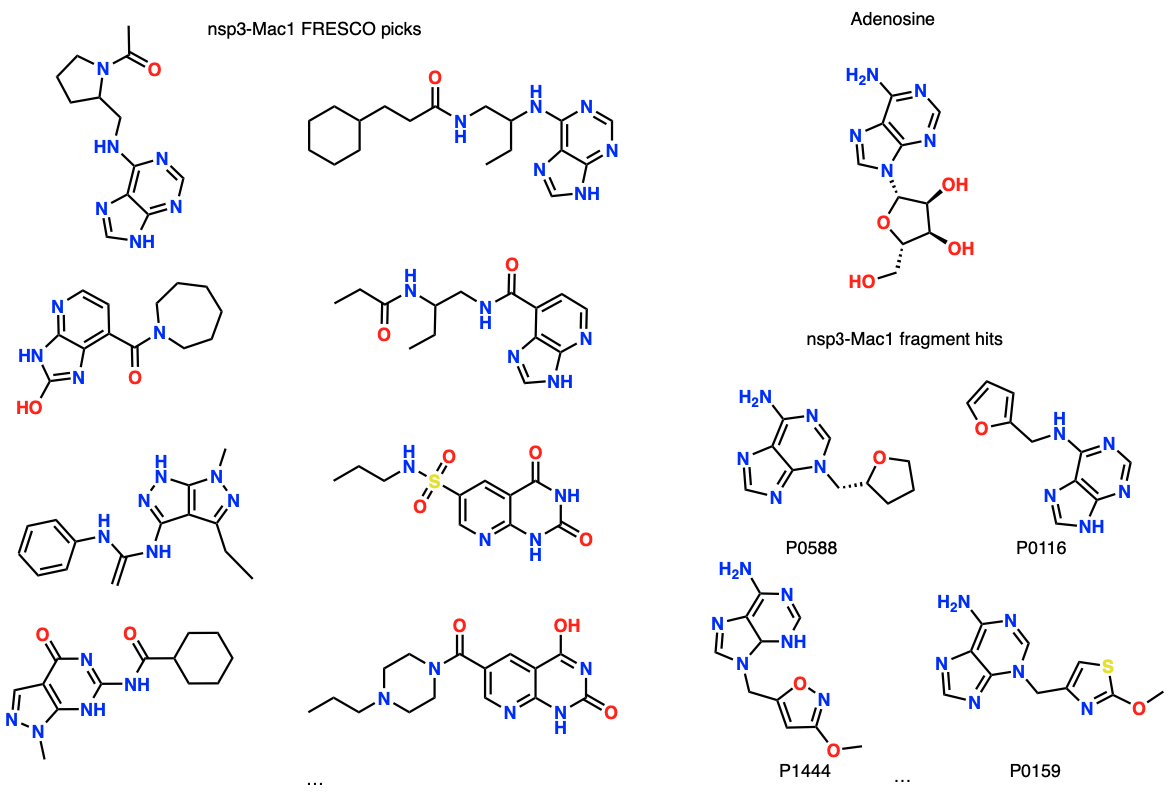
\includegraphics[width=0.8\linewidth]{Chapters/Fresco/Figs/mac1_ligands.png}
 \caption{\textbf{Top-ranked compounds from FRESCO mimic the natural substrate of nsp3-Mac1.} The molecules favoured by FRESCO tend to contain an acceptor-donor pair spatially proximal to a heterocyclic motif. This mimics adenosine, a core in the natural substrate. This motif is also shared in many of the initial fragment hits, with some example structures shown in the figure.}
 \label{fig:mac1_ligands}
\end{figure}

Repeating the FRESCO workflow on a fragment screen against Mac1 \cite{Schuller2021Mac1Frag}, we obtained 22358 clusters of top-ranked compounds and successfully made 52 molecules. We find that the molecules favored by FRESCO tend to contain a HBA-HBD pair that is spatially proximal within a heterocyclic motif. This mimics adenosine, a core in the natural substrate, and this motif is shared in many of the initial fragment hits (Figure \ref{fig:mac1_ligands}). We successfully ordered and assayed 52 of the compounds identified by FRESCO (see SI for the whole library). Two of the compounds show non-negligible activity at high concentration - at 250\uM, compound Z5551425673 (as a racemic mixture) has an inhibition of 30.1\%, while compound Z1102995175 has 24.8\%.

\begin{figure}[!t]
 \centering
 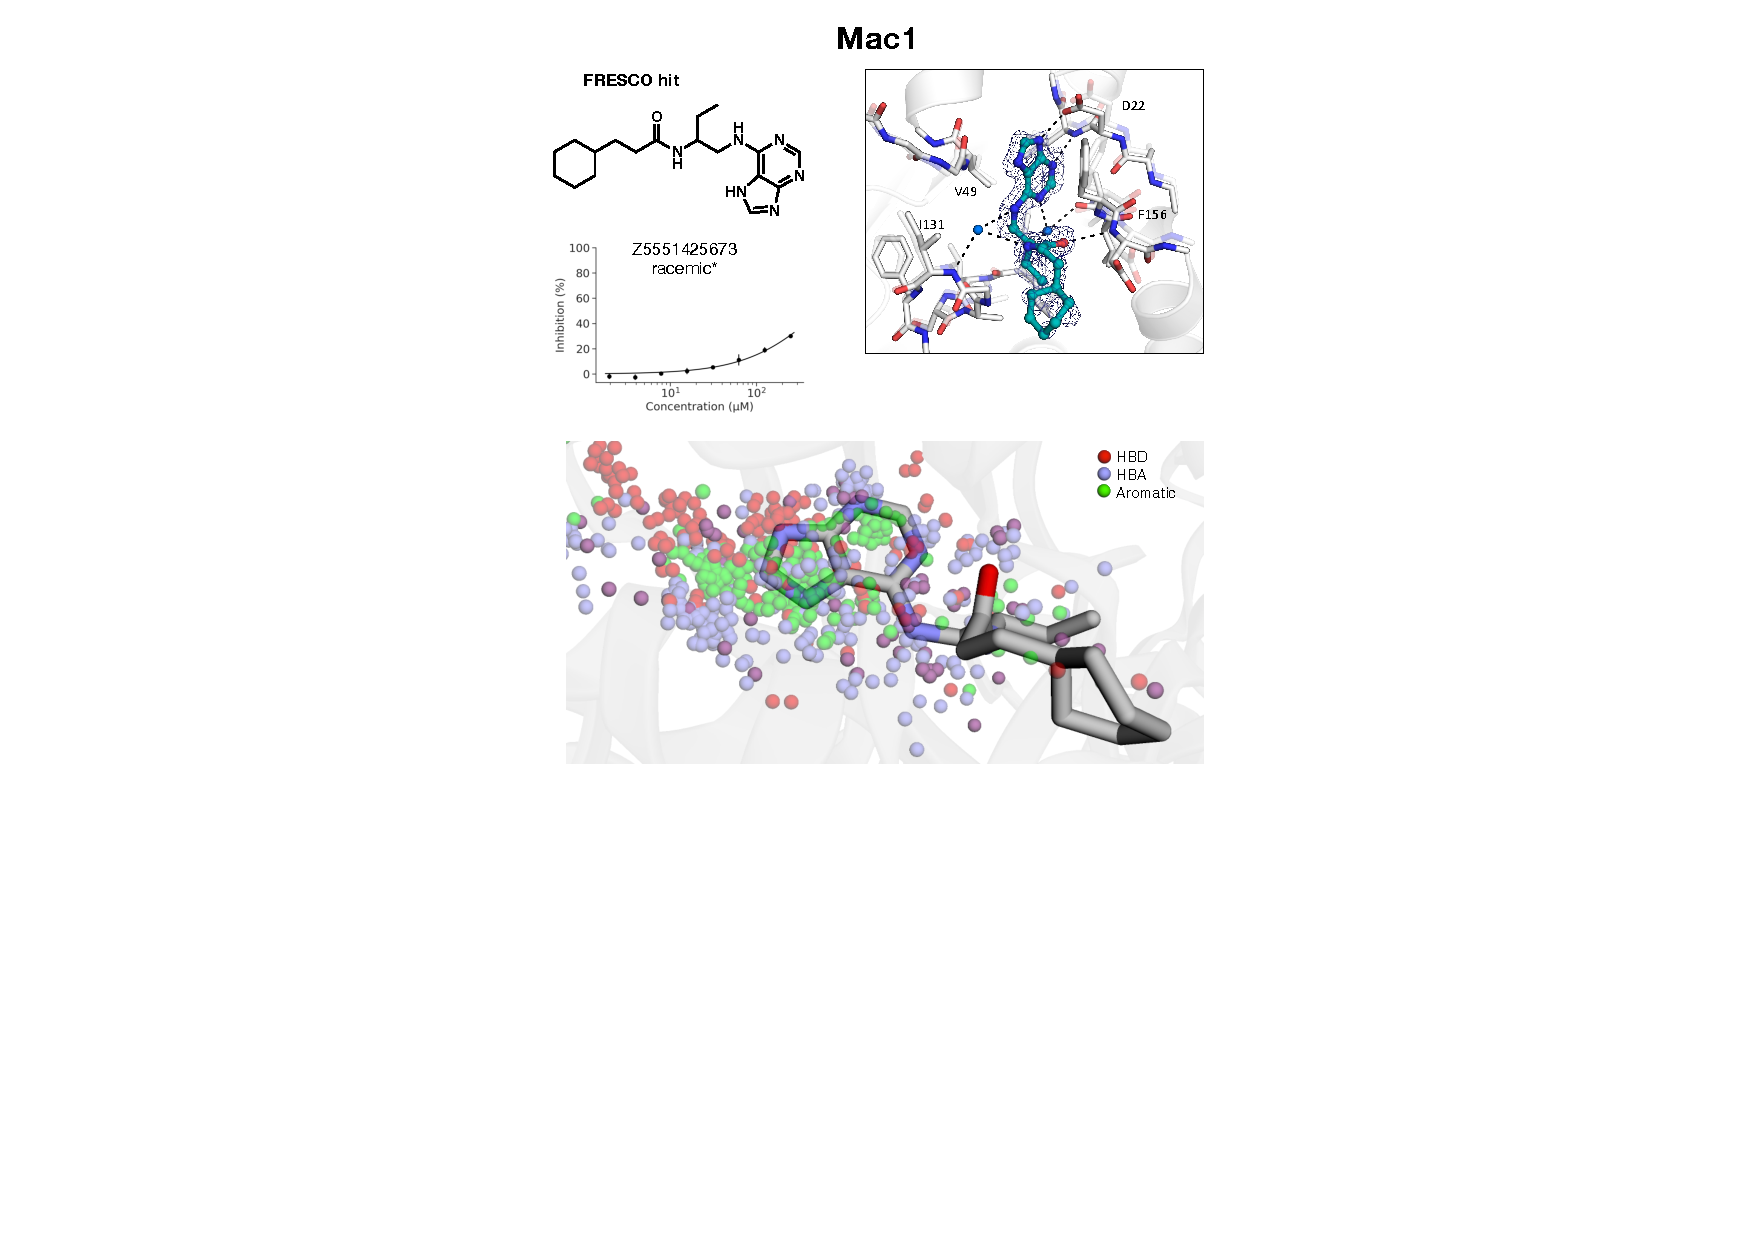
\includegraphics[width=0.75\linewidth]{Chapters/Fresco/Figs/mac1_fig.pdf}
 \caption{\textbf{FRESCO identifies a hit against nsp3-Mac1 with structural confirmation.} (\textbf{a}) Compound Z5551425673 is identified as a hit against Mac1 via HTRF assay, with (\textbf{b}) hit confirmation via resolution of a crystal structure of Z5551425673 (colored in cyan) bound to the Mac1 active site. (\textbf{c}) The pharmacophores of Z5551425673 match those exhibited by the fragment hits as highlighted by overlaying the bound structure of Z5551425673 (PDB 7FR2) on the distribution of pharmacophores from the fragment ensemble. Note that some functional groups can be regarded as both hydrogen-bond acceptor (blue) and hydrogen-bond donor (red) pharmacophores and hence they are illustrated as purple.}
 \label{fig:mac1_hit}
\end{figure}

In addition, an X-ray crystallographic screen was also run on the compounds revealing the structure of Z5551425673 (as the S-stereoisomer) bound to the active site (Figure \ref{fig:mac1_hit}). Crystal structures of 9 other compounds chosen via the FRESCO workflow were also obtained though they did not show notable inhibition via HTRF assay. The orthogonal experimental assay and crystal structure results confirm that Z5551425673 is a hit. 

As with Mpro, 11 close analogues to Z5551425673 were ordered to explore the structure-activity relationship of the hit and ensure that the compound is not a singleton. 4 compounds perturbing the aliphatic tail substructure had relatively negligible effect while the remaining compounds perturbing the purine group led to a large drop in activity (Figure \ref{fig:mac1_rounds}). These sets of molecules, still weak in potency, are potentially promising starting points for a hit expansion campaign. 

\begin{figure}[!t]
 \centering
 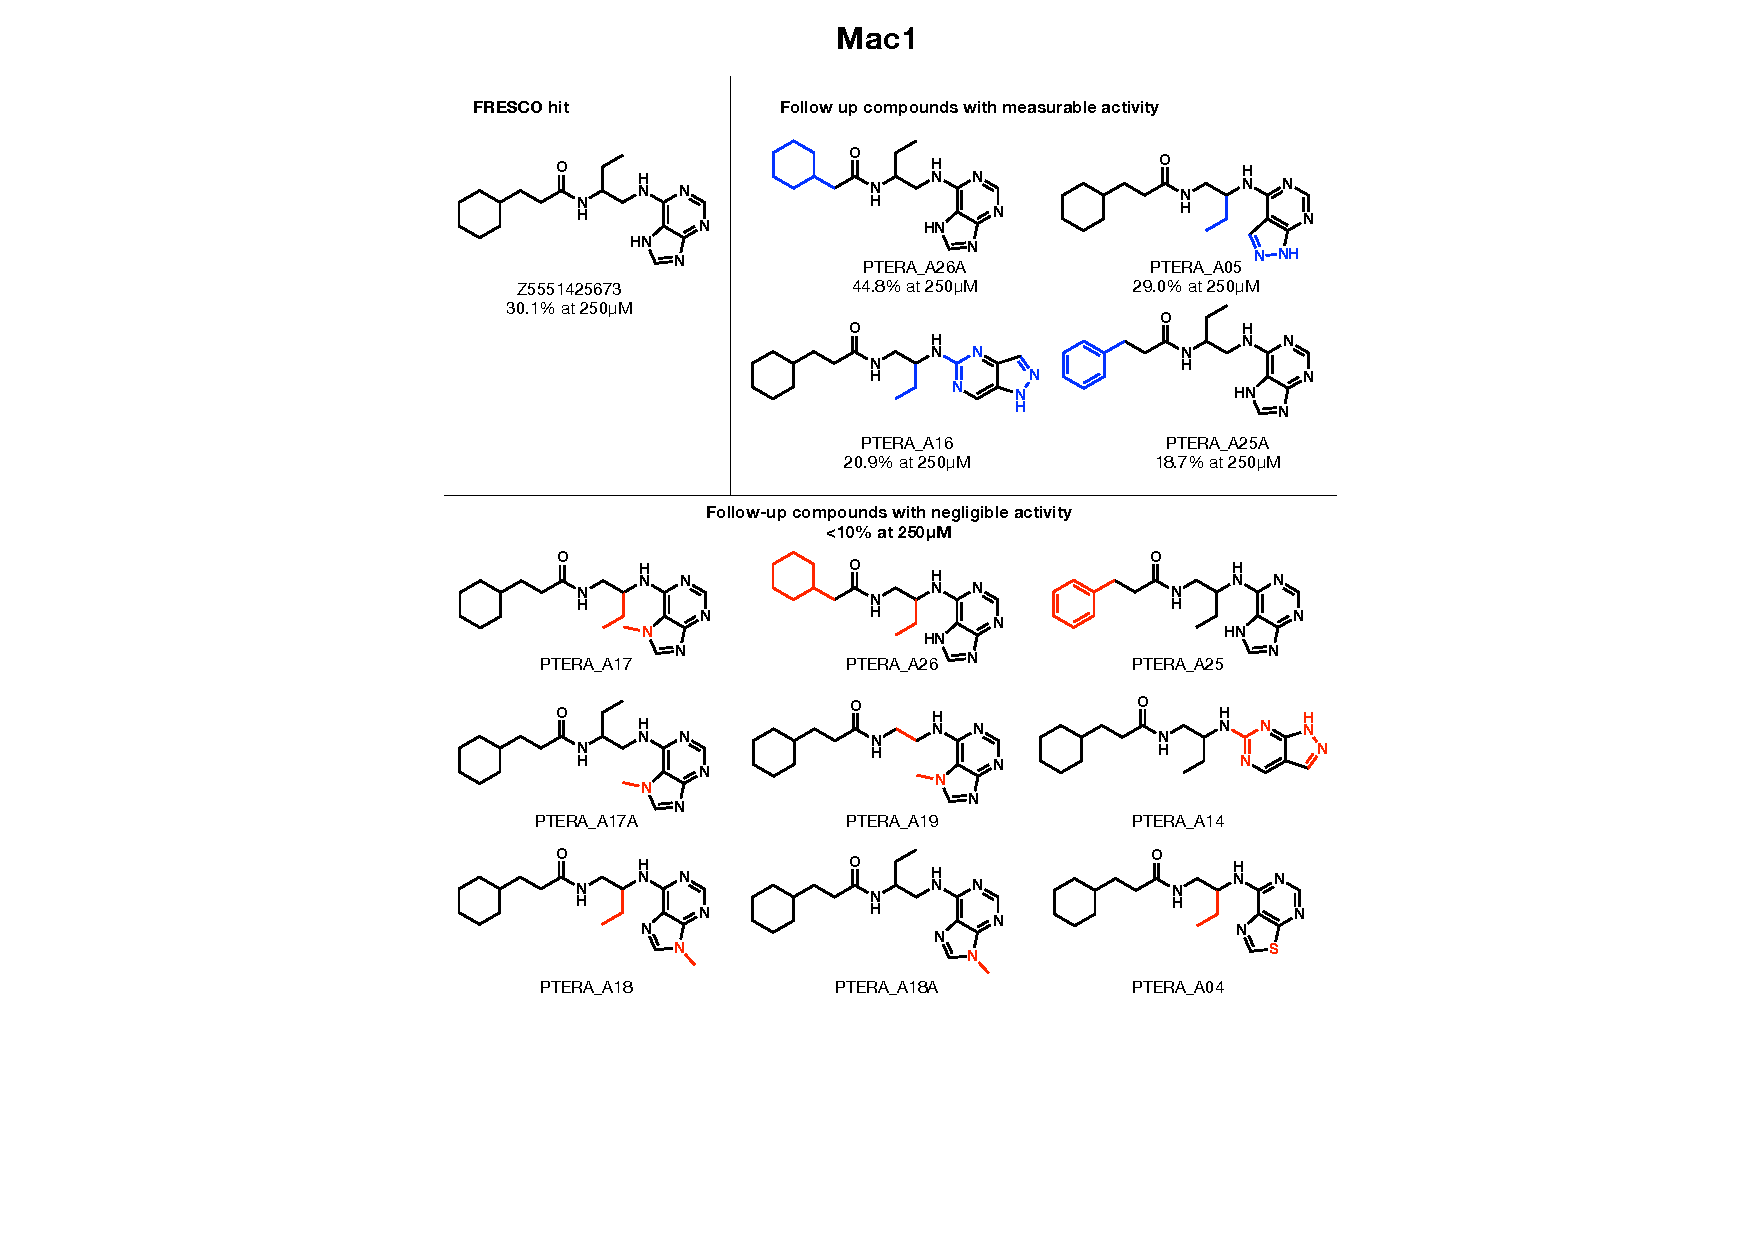
\includegraphics[width=0.75\linewidth]{Chapters/Fresco/Figs/mac1_rounds.pdf}
 \caption{\textbf{nsp3-Mac1 hit confirmation via determination of structural-activity relationship.} Close analogues around the hit compound identified by FRESCO, Z5551425673, reveals structure-activity relationship which derisks singleton artefacts.}
 \label{fig:mac1_rounds}
\end{figure}


\section{Discussion} \label{sec:fresco_discussion}

Here we show that the combination of computational statistics with high-throughput structural biology and large libraries of purchasable fragment-like molecules unlocks a powerful tool in hit discovery. Going beyond classical fragment-based drug design, which involves merging or expanding a small set of fragments, we derived a statistical framework that leverages dense fragment hits to build potent inhibitors. Whilst individual fragments are weak binders, our key insight is that a fragment-protein interaction is likely to be significant if multiple fragments are making similar interactions. Therefore, by picking out these persistent interactions, we can discern the salient chemical motifs which make favourable interactions with the binding site. Specifically, we coarse-grained fragments into pharmacophores, and infer the distribution of pairwise distances between pharmacophores using Kernel Density Estimation. We then screen large libraries of purchasable compounds against this fragment-derived pharmacophore distribution. We retrospectively validated our method using data from The COVID Moonshot, an open science drug discovery campaign against the SARS-CoV-2 main protease and prospectively discovered new hits against SARS-CoV-2 main protease and nsp3-Mac1.

%Although there has been rapid growth in employing machine learning for drug discovery in recent years, particularly in QSAR/molecular property prediction, the vast majority of machine learning approaches are supervised learning techniques. These methods require not merely the existence of experimental assay data, but its existence in sufficient quantity and quality to train a useful model. The nature of the problem of hit detection in early-stage drug discovery is one where such data is nonexistent, which is a fundamental obstacle to applying current techniques. This works shows how we can instead tap into an underutilised source of rich data by employing unsupervised learning on structural data for affinity prediction. There is already a wealth of crystallographic data available and through collaboration with experimentalists, the field of structural biology can provide a wealth of unique informative unlabelled data for building useful machine learning models for drug discovery.

More generally, we note that our method does not require the observation of affinity data in order to infer potency. This is done by employing an unsupervised machine learning approach on unlabelled structural biology data. As the throughput of structural biology increases, we hope that an unsupervised approach may unlock novel ways of overcoming data limitations in the protein-ligand affinity prediction problem.

Finally, although prospective studies demonstrated FRESCO's ability to identify hits, we note that the hit rate and potency of the identified hits are both lower than the retrospective experiments. This highlights the importance of prospective validation in machine learning -- retrospective studies are biased by the fact that the model is re-scoring ``reasonable'' design from medicinal chemists, whereas in prospective evaluations, the model is used to score the large chemical space without further inductive biases. Future efforts to improve FRESCO should seek to include further inductive biases, for example, incorporating physics-based constraints such as docking to filter FRESCO outputs, as well as solidifying a human-in-the-loop approach to select top hits. 